\documentclass[12pt,a4paper,openany]{report}
\usepackage{graphicx}
\usepackage[english]{babel}
\renewcommand{\thesection}{\arabic{section}}
\usepackage{float}

\title{Faculty of Computing and Informatics\\
TPT1201\\
Research Methodology\\
Assignment 2\\}
\author{ Nur Farah Asylah Bt Nordin \\
1122702103 \\}
\date{\today}

\begin{document}
\maketitle
\pagebreak 
\begin{center}
\Huge {Real Time Water Level Monitoring System and Rise Prediction }\\
\small Nur Farah Asylah Bt Nordin
\end{center}

\section{Executive Summary}
Flood events has been a great concern for the people residing near the reservoir or any stream rivers. Flood causes loss of lives and damages to the buildings and homes of the surrounding area. Therefore, a reliable and accurate water level monitoring and prediction system is much needed as the occurrence of this event is unpredictable and sudden. The objectives of this research is to provide accurate water level prediction results using a real time monitoring system. Three IP cameras will be set up at the different connecting rivers to obtain the image of the water gauges. These images will then undergo Thresholding method and Character recognition method to obtain the water line and character value. The actual value of the water level will then be obtained from Interpolation method which combines the two filtered images. After the images from the three monitoring devices has been recognized, the values will then be used for the prediction of rising of water level by using Nonlinear Autoregressive with Exogenous Input (NARX) model. This experiment will be conducted in three consecutive days to record and measure the variations of the water level. The results will be mapped to a graph and be compared with the observed values to compute the significance of both values. With this proposed method, the system able to provide a real time monitoring water level and also the water level rise prediction which can lead to floods. The system is expected to provide the public with the condition of the river water level and be aware of the river activities.




\section{Introduction}
Real time monitoring system has helped many area fields in term of detection and prevention. Typically, this system would be applied to a video surveillance cameras or Closed-circuit television (CCTV) to monitor a certain area in buildings or homes. In (Kim, Park, Lee, Kim, & Seo, 2014) proved that CCTV could also be used for measurement of water level. The measurement was evaluated by using automatic image processing on the captured images. The Image Water Level Gauge is a technology that combines video surveillance and water level measurement without needing any additional water level sensor equipment.
With this values obtained, the system able to compute the prediction on the rising of water level using Nonlinear Autoregressive with Exogenous Input (NARX).
\section{Justification of Research}
Recent event, a massive flood has strike Kelantan which is the north east of Peninsular Malaysia. Eastern Malaysia suffers from annual flooding. Apparently, this was the worst case in the history of the state due to the strong winds and heavy rainfall. This event also had distributed across the country towards southern Thailand.
\par Therefore, an accurate flood water level prediction is very important in flood modelling because it can give ample time to residents nearby flood location for evacuation purposes. 
\section{Research Objectives}
\begin{itemize}
\item To provide accurate results and reliable real time water monitoring system. 
\item To provide prediction of the rising of water level .
\end{itemize}



\section{Literature Review}
Artificial Neural Network (ANN) able to solve complex nonlinear system without the needs of any physical knowledge of the system (Ruslan, Samad, Zain, & Adnan, 2014).One class of ANN is Nonlinear Autoregressive with Exogenous Input (NARX) .The NARX model was developed based on Autoregressive with Exogenous Input (ARX) which represents linear system identification model. In (Ruslan, Samad, Md Zain, & Adnan, 2013), a comparative study between the two models, Multiple Input Single Output (MISO) ARX model and NARX model was conducted . The study had shown that the NARX model shows better performance compare to MISO ARX and gives high degree of accuracy.On a recent study conducted here in Malaysia, NARX model has been used for the prediction of flood water level 5 hours in advance (Adnan, Samad, Zain, & Ruslan, 2014).  Implementation of the NARX model had shown satisfactory performance in comparing the predicted value to the actual water level.  Therefore, the use of NARX model is convincing for this study.




\section{Research Methodology}
\subsection{NARX Model}
The equation of the NARX model is given at Equation (1).

\begin{equation}
y(t) = f(y(t-1),...y(t-n),u(t-1),...u(t-m)) + e(t)
\end{equation}

$e(t)$ is the white noise residuals and the next value of dependent output signal, $y(t)$ is regressed on previous values of the output signal and previous values of an independent (exogenous) input signal.  
In this study, the equation in is used instead which was the extraction from the equation in (Ruslan et al., 2014)
\begin{figure}[H]
\centering
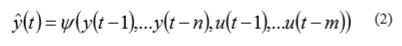
\includegraphics[scale=0.8]{./images/eq}
\end{figure}

There are two architectures in NARX network which is the parallel (P) and series-parallel (SP) architectures. However, the series-parallel architecture offer advantages of feed-forward architecture. In Figure 2 shows how the inputs being constructed to produce the predicted outputs using Series-Parallel NARX architecture (Ruslan et al., 2013).
\begin{figure}[H]
\centering
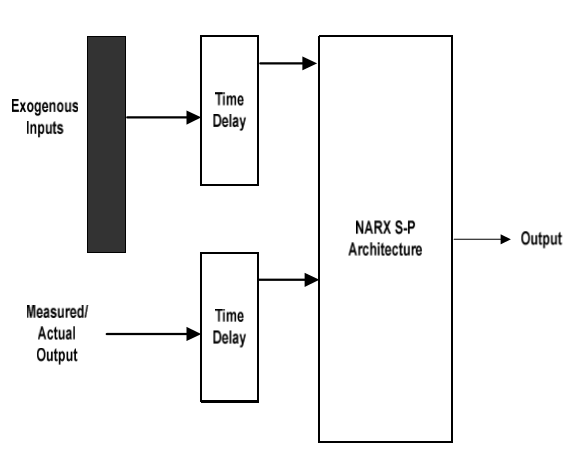
\includegraphics[scale=0.6]{./images/SPNARX}
\caption {Series-Parallel NARX architecture}
\end{figure}




\subsection{Technique}
Three high-resolution monitoring IP cameras will be used for this study. One of them will be installed at the susceptible area while the other cameras will be at the two upstream rivers.IR lighting also will be attached to it to provide brighter vision during the night. The cameras will capture the water gauge of the bridge. The captured images will be transmitted to the local server through the network. The images will then processed in real-time. Two methods will be used in order to obtain the water level of the gauge. One method involve character recognition while another is to obtain the water line detection. These method will run concurrently and the output will be processed into an interpolation method to calculate the actual height of the water gauge. This processes can be represented in Figure 2 (Lin et al., 2013).
\begin{figure}[H]
\centering
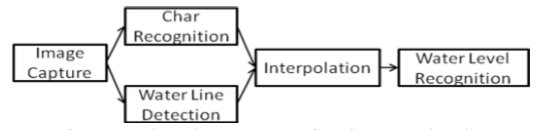
\includegraphics[scale=0.8]{./images/WaterLvl}
\caption {Flowchart to recognize the water level}
\end{figure}

With the obtained water level from the three measured area, these values will be the input to the NARX model to predict the water level ahead of time. Figure 4 shows the block diagram of the NARX structure.
\begin{figure}[H]
\centering
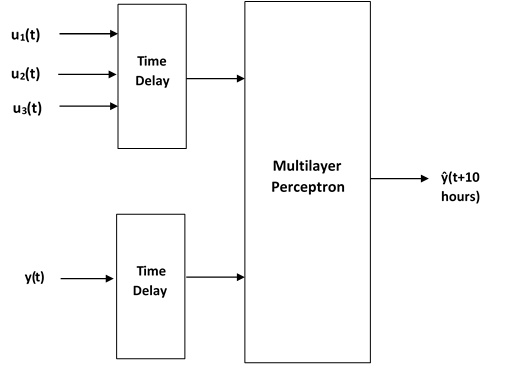
\includegraphics[scale=0.6]{./images/NARX}
\caption{NARX architecture}
\end{figure}
\par
$u_{1}(t)$, $u_{2}(t)$ and $u_{3}(t)$ represents the water levels at three upstream rivers and the difference of water levels at the main location due to rainfall. y(t) represents water levels at the main location. 
The output of the NARX model represents the predicted water level which will then be constructed in to a table and plotted in to a graph. This results from this experiment is measured for three consecutive days. Based on the graph plotted, the prediction time also able to be obtained by the delay steps of NARX model. Each steps represented 10 minutes time interval. With this results, warn could be released to those within the susceptible area so that they are prepared ahead of time when the water level reaches the critical level.
In order to determine the accuracy of this method, the predicted values and the observed values will be mapped together to compare the significance. Figure  shows the flowchart of the whole process of real-time monitoring and rise prediction of water level.

\begin{figure}[H]
\centering
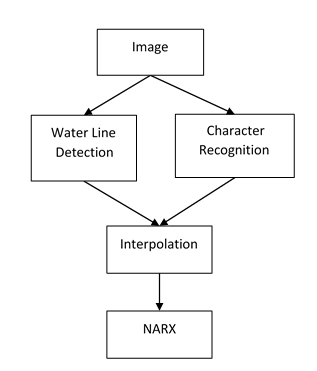
\includegraphics[scale=0.8]{./images/flowchart}
\caption{Flowchart real-time monitoring and rise prediction of water level}
\end{figure}

\section{References/Bibliography}
\par
Adnan, R., Samad, A. M., Zain, Z. M., & Ruslan, F. A. (2014). 5 hours flood prediction modeling using improved NNARX structure: case study Kuala Lumpur. In System Engineering and Technology (ICSET), 2014 IEEE 4th International Conference on (Vol. 4, pp. 1–5). IEEE. Retrieved from \\ http://ieeexplore.ieee.org/xpls/abs_all.jsp?arnumber=7111799 \\
\par
Kim, Y., Park, H., Lee, C., Kim, D., & Seo, M. (2014). Development of a Cloud-based Image Water Level Gauge. IT CoNvergence PRActice (INPRA), 2(1), 21–28.\\
\par
Lin, F., Chang, W.-Y., Lee, L.-C., Hsiao, H.-T., Tsai, W.-F., & Lai, J.-S. (2013). Applications of Image Recognition for Real-Time Water Level and Surface Velocity (pp. 259–262). IEEE. http://doi.org/10.1109/ISM.2013.49 \\
\par
Ruslan, F. A., Samad, A. M., Md Zain, Z., & Adnan, R. (2013). Multiple Input Single Output (MISO) ARX and NARX model of flood prediction system: A comparative study. In Control System, Computing and Engineering (ICCSCE), 2013 IEEE International Conference on (pp. 254–258). IEEE. Retrieved from http://ieeexplore.ieee.org/xpls/abs_all.jsp?arnumber=6719969\\
\par
Ruslan, F. A., Samad, A. M., Zain, Z. M., & Adnan, R. (2014). Flood water level modeling and prediction using NARX neural network: Case study at Kelang river. In Signal Processing & its Applications (CSPA), 2014 IEEE 10th International Colloquium on (pp. 204–207). IEEE. Retrieved from \\ http://ieeexplore.ieee.org/xpls/abs_all.jsp?arnumber=6805748 \\
\par

\end{document}
